%%%%%%%%%%%%%%%%%%%%%%% file template.tex %%%%%%%%%%%%%%%%%%%%%%%%%
%
% This is a general template file for the LaTeX package SVJour3
% for Springer journals.          Springer Heidelberg 2010/09/16
%
% Copy it to a new file with a new name and use it as the basis
% for your article. Delete % signs as needed.
%
% This template includes a few options for different layouts and
% content for various journals. Please consult a previous issue of
% your journal as needed.
%
%%%%%%%%%%%%%%%%%%%%%%%%%%%%%%%%%%%%%%%%%%%%%%%%%%%%%%%%%%%%%%%%%%%
%
% First comes an example EPS file -- just ignore it and
% proceed on the \documentclass line
% your LaTeX will extract the file if required
\begin{filecontents*}{example.eps}
%!PS-Adobe-3.0 EPSF-3.0
%%BoundingBox: 19 19 221 221
%%CreationDate: Mon Sep 29 1997
%%Creator: programmed by hand (JK)
%%EndComments
gsave
newpath
  20 20 moveto
  20 220 lineto
  220 220 lineto
  220 20 lineto
closepath
2 setlinewidth
gsave
  .4 setgray fill
grestore
stroke
grestore
\end{filecontents*}
%
\RequirePackage{fix-cm}
%
\documentclass{svjour3}                     % onecolumn (standard format)
%\documentclass[smallcondensed]{svjour3}     % onecolumn (ditto)
%\documentclass[smallextended]{svjour3}       % onecolumn (second format)
%\documentclass[twocolumn]{svjour3}          % twocolumn
%
\smartqed  % flush right qed marks, e.g. at end of proof
%
\usepackage{graphicx}
\usepackage{epstopdf}
\usepackage{subfigure}

\usepackage{mathptmx}

\usepackage{times}

\usepackage{algorithm}% http://ctan.org/pkg/algorithm
\usepackage{algpseudocode}% http://ctan.org/pkg/algorithmicx

\usepackage{url}

\usepackage{color, xcolor}
\definecolor{darkg}{rgb}{0,0.6,0}
\definecolor{lgreen}{rgb}{0,0.8,0}
\definecolor{purple}{rgb}{0.93,0.48,0.03}
\definecolor{orange}{rgb}{0.43,0.48,0.03}
% \ifdraft
%Our comments:
\newcommand{\lmc}[1]{{\color{lgreen}[LM: #1]}}
\newcommand{\wqc}[1]{{\color{orange}[WQ: #1]}}
\newcommand{\wq}[1]{{\color{blue}#1}}
\newcommand{\lm}[1]{{\color{darkg}#1}}

\newcommand{\m}{\textcolor{black}}

\usepackage{multirow}
\usepackage{tabularx}

\usepackage{algpseudocode}
\usepackage{natbib}
\usepackage[misc]{ifsym}

\begin{document}

\title{Unfolding the City: \wq{Exploring Urban Spatial Attractiveness with Individual Characteristics}}
%\thanks{Grants or other notes
%about the article that should go on the front page should be
%placed here. General acknowledgments should be placed at the end of the article.}

%\subtitle{Do you have a subtitle?\\ If so, write it here}

%\titlerunning{Short form of title}        % if too long for running head

\author{Qi Wang \and Min Lu \and Yang Yue \and Qingquan Li}

%\authorrunning{Short form of author list} % if too long for running head

\institute{Q. Wang \and Q. Li(\Letter) \at
              the State Key Laboratory of Information Engineering in Surveying, Mapping and Remote Sensing, Wuhan University, Wuhan, China, and also ShenZhen Key Laboratory of Spatial Smart Sensing and Services, ShenZhen University, Shenzhen 518060, China \\
              Tel.: +86-13297983047\\
              \email{wangqi@whu.edu.cn}, {liqq@szu.edu.cn}           %  \\
           \and M. Lu \and Y. Yue \at
              School of Architecture and Urban Planning, and also ShenZhen Key Laboratory of Spatial Smart Sensing and Services, ShenZhen University, Shenzhen 518060, China \\
              \email{minlu@szu.edu.cn}, {yueyang@szu.edu.cn}           %  \\
}

\date{Received: date / Accepted: date}
% The correct dates will be entered by the editor


\maketitle

\begin{abstract}
A city is shaped not only by its assembled infrastructures but also the people living inside it. People in a wide range of individual characteristics visit places with different weights and preferences, sculpturing the city into a space of diverse mobility patterns. Different from the well study of anonymous travel behaviors, the mobility patterns of characterized individuals, is less studied because of the challenges in collection and analysis of data with privacy. In this work, we take a step forward and perform an online census to collect individual profiles and movements from large-scale volunteers. Then we develop a visual analytic system to investigate the mobility patterns of groups by specifying characteristics. To facilitate the identification of characterized groups, individuals are embedded in t-SNE projection for an abstract overview as well as drawn as vivid graphics by a data-driven profile method for detail examination. A 2.5D spatial visualization is proposed to maintain a compact multivariable analysis by relaxing the z-axis to encode information, such as visiting frequency, demands, traveling distance, etc. Together with the cross-filter and flexible 2.5D interactions, the effectiveness and usability of the system are well demonstrated by a study made in Shenzhen.

\keywords{Visual analytics \and mobility pattern \and individual characteristics \and city }
% \PACS{PACS code1 \and PACS code2 \and more}
% \subclass{MSC code1 \and MSC code2 \and more}
\end{abstract}

\section{Introduction}
\iffalse
What is it that makes some places, regions or nations appear more attractive than others to live in, visit or invest in? Does it depend on the particular characteristics or situation of the persons considering the attractiveness, in what phase in life the persons find themselves, or are there some common features, perhaps place characteristics that are viewed positively by all, independently of context?



\fi


\label{intro}
\wqc{change mobility pattern to spatial attractiveness}\\
The science fiction \textit{Folding Beijing}~\citep{hao2016_foldingbeijing} depicts a world where three classes of people live in independent spatial-temporal patterns, though sharing the same earth surface. This is an artistical metaphor for one potential fact that people make different decisions in visiting places according to individual determinants, such as social, economic, educational factors, etc. This phenomenon has attracted the research interest for a long time in the sociological field. Back to 1970, Pahl~\citep{pahl1975whose} posed the question `whose city` and interest in understanding the territorial inequalities. Contemporary contestation also continually raise the banner `The City Belongs to All!'~\citep{Mayer2017_whosecity}. Having a good understanding of how the mobility patterns relate to characterized individuals sheds light on region utilization, diversity mix-up, and opportunities promotion.

In the past decades, the power of visual analytics in exploring spatial-temporal data has been recognized and well developed. Transportation problems are answered by various movement data, such as traffic jams in taxi GPS trajectoires~\citep{wang2013visual}, interchanging flows in public transportation~\citep{zeng2013visualizing}, etc. The presence of social media applications fuels the spatial analysis with rich semantic texts, so researchers get the chances to explore the thematic meaning of the moving behavior, such as events~\citep{chen2017map} or topics~\citep{bosch2013scatterblogs2}. Those works essentially contribute in deepening the contextual understanding of moving activity. But they rarely combine the mobility with individuals' characteristics because which cannot be 100\% inferred from social media profiles. There is still a research gap in exploring the relationship between mobility pattern and characteristics.


In this work, we contextualize the analysis of mobility pattern in the backcloth of individual characteristics. Our motivation is to fuse the movement data with individuals' profiles in an attempt to ascertain the dynamics pattern of groups with different characteristics. To this, we need to get the characterized information of movers. The sensitivity issue in privacy data is one of the main challenges. The conventional offline census takes lots of effort and too much time to be out of date. With the wide use of the mobile device, it is possible to count information online. In this work, with a census survey released via social media application, we ran an online demographical collection campaign. Then we developed a visual analytics system to explore the mobility patterns centered around people. The system incorporates visualizations of individuals' characteristics, including t-SNE for an overview and data-driven profile visualization for the detailed check, as well as 2.5D spatial visualization to explore the mobility patterns. Finally, applying our method in Shenzhen, several cases are derived to demonstrate the powers of our method. There are two contributions of this work:

(1) investigate mobility patterns with characteristics, which is a natural step into research of social understanding of the city.

(2) develop a visual analytic system, whose effectiveness and usability is well demonstrated by a study made in Shenzhen.



\section{Related work}

This work concerns the research topic of spatial data visual analytics. Spatio-temporal data has three components, i.e., spatial, temporal and thematic~\citep{andrienko2013visual}. Lots of related work focus on the spatio-temporal analysis in movement data, in the absence of thematic information. The presence of geotagged social media data flourishes the exploration of thematic information along with movement. By analyzing the texts, those work explain what drive the moving activities or what is resulted from. This work continues the thematic research in movement data but focuses more on individual characteristics. Landed by a census experiment, this work is able to analyze the profile information directly, to get rid of indirect data inferred from social media data as other related works do.

\subsection{Movement data analysis}
 With the development of location-acquisition techniques, massive spatial trajectories are collected, to keep track of the trajectories of various moving objects. Many techniques have been proposed to process, mine trajectory~\citep{Zheng2015_trajectory}. In the field of visualization and visual analytics, spatial visualizations are specifically designed for the time, locations, spatial-temporal information and other properties in the traffic data~\citep{chen2015survey}. A large number of visual analytics tools and applications cover situation-aware exploration, pattern discovery and traffic situation monitoring. Wang et al~\citep{wang2013visual} extract the traffic jam propagation graph extraction to reveal underlying data patterns. Guo et al.~\citep{guo2011tripvista} and Zeng et al.~\citep{zeng2013visualizing} construct geographical regions and visually aggregate the in-between movements as flows. To discover the route travel patterns, Lu et al.~\citep{lu2015trajrank} propose TrajRank to explore the route travel behavior based on ranking. For multiple routes, Liu et al.~\citep{liu2011_routediversity} study the route diversity between locations and Lu et al.~\citep{Lu2017_multipleroute} explore the route choice behavior among multiple routes.

\subsection{Geo-tagged Social Media Data Analysis}
As the presence of social media services, social media data with geo-tags are collected to track people's movements in daily lives. As an analog of remote sensing data in social science research, the geospatial big data has been proposed as social sensing ~\citep{liu2015social}. Hence, analyzing movement information along with rich text has become a hot research area in recent years. Those works infer thematic information from the semantic texts. Cao et al.~\citep{cao2012whisper} propose \textit{Whisper} for tracing the pathways of tweets on a spatial hierarchical layout, to investigate how information flow among multiple places. Krueger et al.~\citep{krueger2014visual} used GPS and location-based service data to support the analysis of movement behaviors. Chen et al.~\citep{chen2016interactive} present a visual analytics system to support the exploration of sparsely sampled trajectory from social media. Some other researchers tend to infer real information, such as names, gender, etc, from social media data~\citep{peddinti2014internet}, to break down the demographic characteristics of social media users. Luo et al.~\citep{luo2016explore} derive race, gender, and age as three demographics dimensions to analyze its impact on the urban human mobility patterns. Since real information is not enforced in social media, the wrong inferring is inevitable. Longley et al.~\citep{Longley2015}~\citep{Paul2016_twitter} identifies and assess the biases inherent in social media usage in social research and evaluate the deployment of social media data in research applications.

\section{Online Census}
The advent of mobile sensing techniques and social media applications makes it possible to collect spatial data from the social media source. Complementary to the conventional census, it brings the benefit of larger sampling frequency and a broader range in terms of space and time. It is possible to reach a wide range of individuals and collect the movement in human inactive time, such as the mid-night.


\begin{figure}[htb!]
 \centering % avoid the use of \begin{center}...\end{center} and use \centering instead (more compact)
 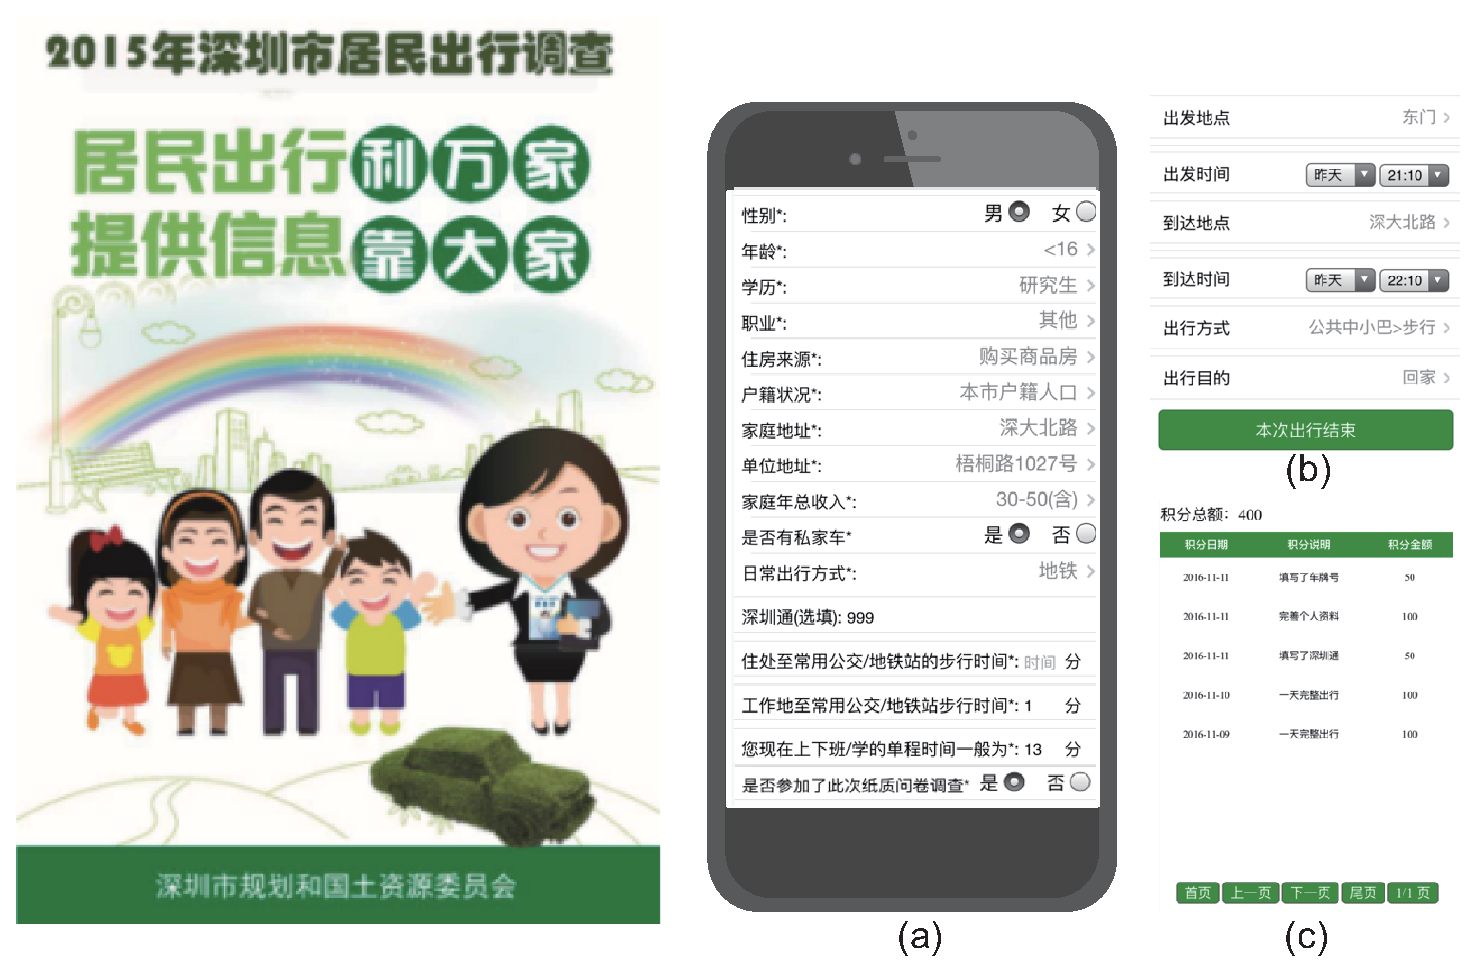
\includegraphics[width=\columnwidth]{pictures/survey_app}
 \caption{Census Interface: (a) personal characteristics collecting page; (b) trips collecting page; (c) credit system page}
 \label{fig:app}
\end{figure}

In this work, we perform the census survey in Shenzhen, which is one of the most modern metropolia in China. The experiment is deployed on Wechat, a widely used social media application. Figure~\ref{fig:app} shows the data collecting interfaces. Each individual hands in his or her personal characteristics. For privacy issue, all detailed personal information are desensitized to categorical levels (Figure~\ref{fig:app}(a)).

\begin{figure}[htb!]
 \centering % avoid the use of \begin{center}...\end{center} and use \centering instead (more compact)
 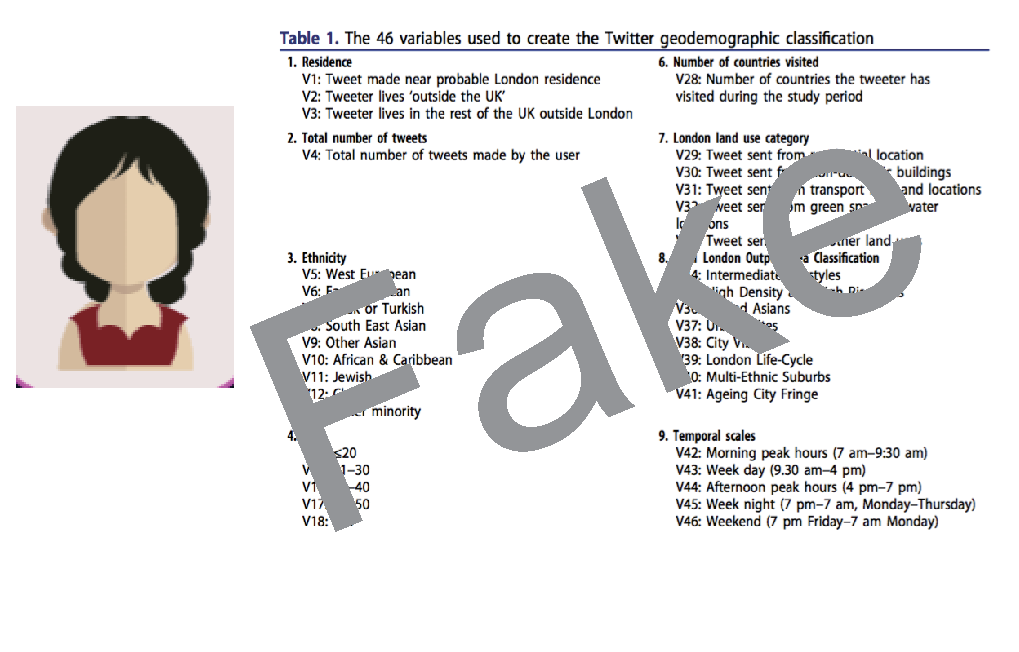
\includegraphics[width=\columnwidth]{pictures/data_over}
 \caption{Profile of Individual: eight individual characteristics enrich the analysis of mobility patterns}
 \label{fig:data_over}
\end{figure}


\textbf{Individual Characteristics} Figure~\ref{fig:data_over} lists the \textit{eight domains}, including social, economic and demographic aspects, to give a generalized description of the individual characteristics. The profile will serve as the ingredients for the analysis of mobility patterns over diverse individuals.

\textbf{Traveling Trips} Besides to those individual characteristics, each individual can upload dynamic traveling trips (Figure~\ref{fig:app}(b)). Each trip requires the information of \textit{start/end location}, \textit{start/end time}, \textit{traveling purpose}. To encourage the trip uploading, a credit system retains the contribution of individuals on trips and rewards the volunteers with the top credits (Figure~\ref{fig:app}(c)).


\subsection{Basic Statistics of Data}

Over the releasing time period from \m{2015-11 to 2016-01}, 21435 individuals (48\% females and 52\% males) were reached and \m{229155} trips are collected. Each volunteer contributes \m{11} trips average.

Our case-study data is confined to a small proportion of Wechat users who opt to contribute their information and trips.
Considering the caveat that self-selecting individuals are most unlikely to represent any clearly defined population~\citep{Longley2015}, we performed a series of preliminary statistics to check whether it is rich enough to represent a wide range of the population in the city.

% In the report (looking for some report), the penetration of mobile device is \m{XXX}, almost every XX people got a Mobile Phone in the urban.

\begin{figure}[htb!]
 \centering % avoid the use of \begin{center}...\end{center} and use \centering instead (more compact)
 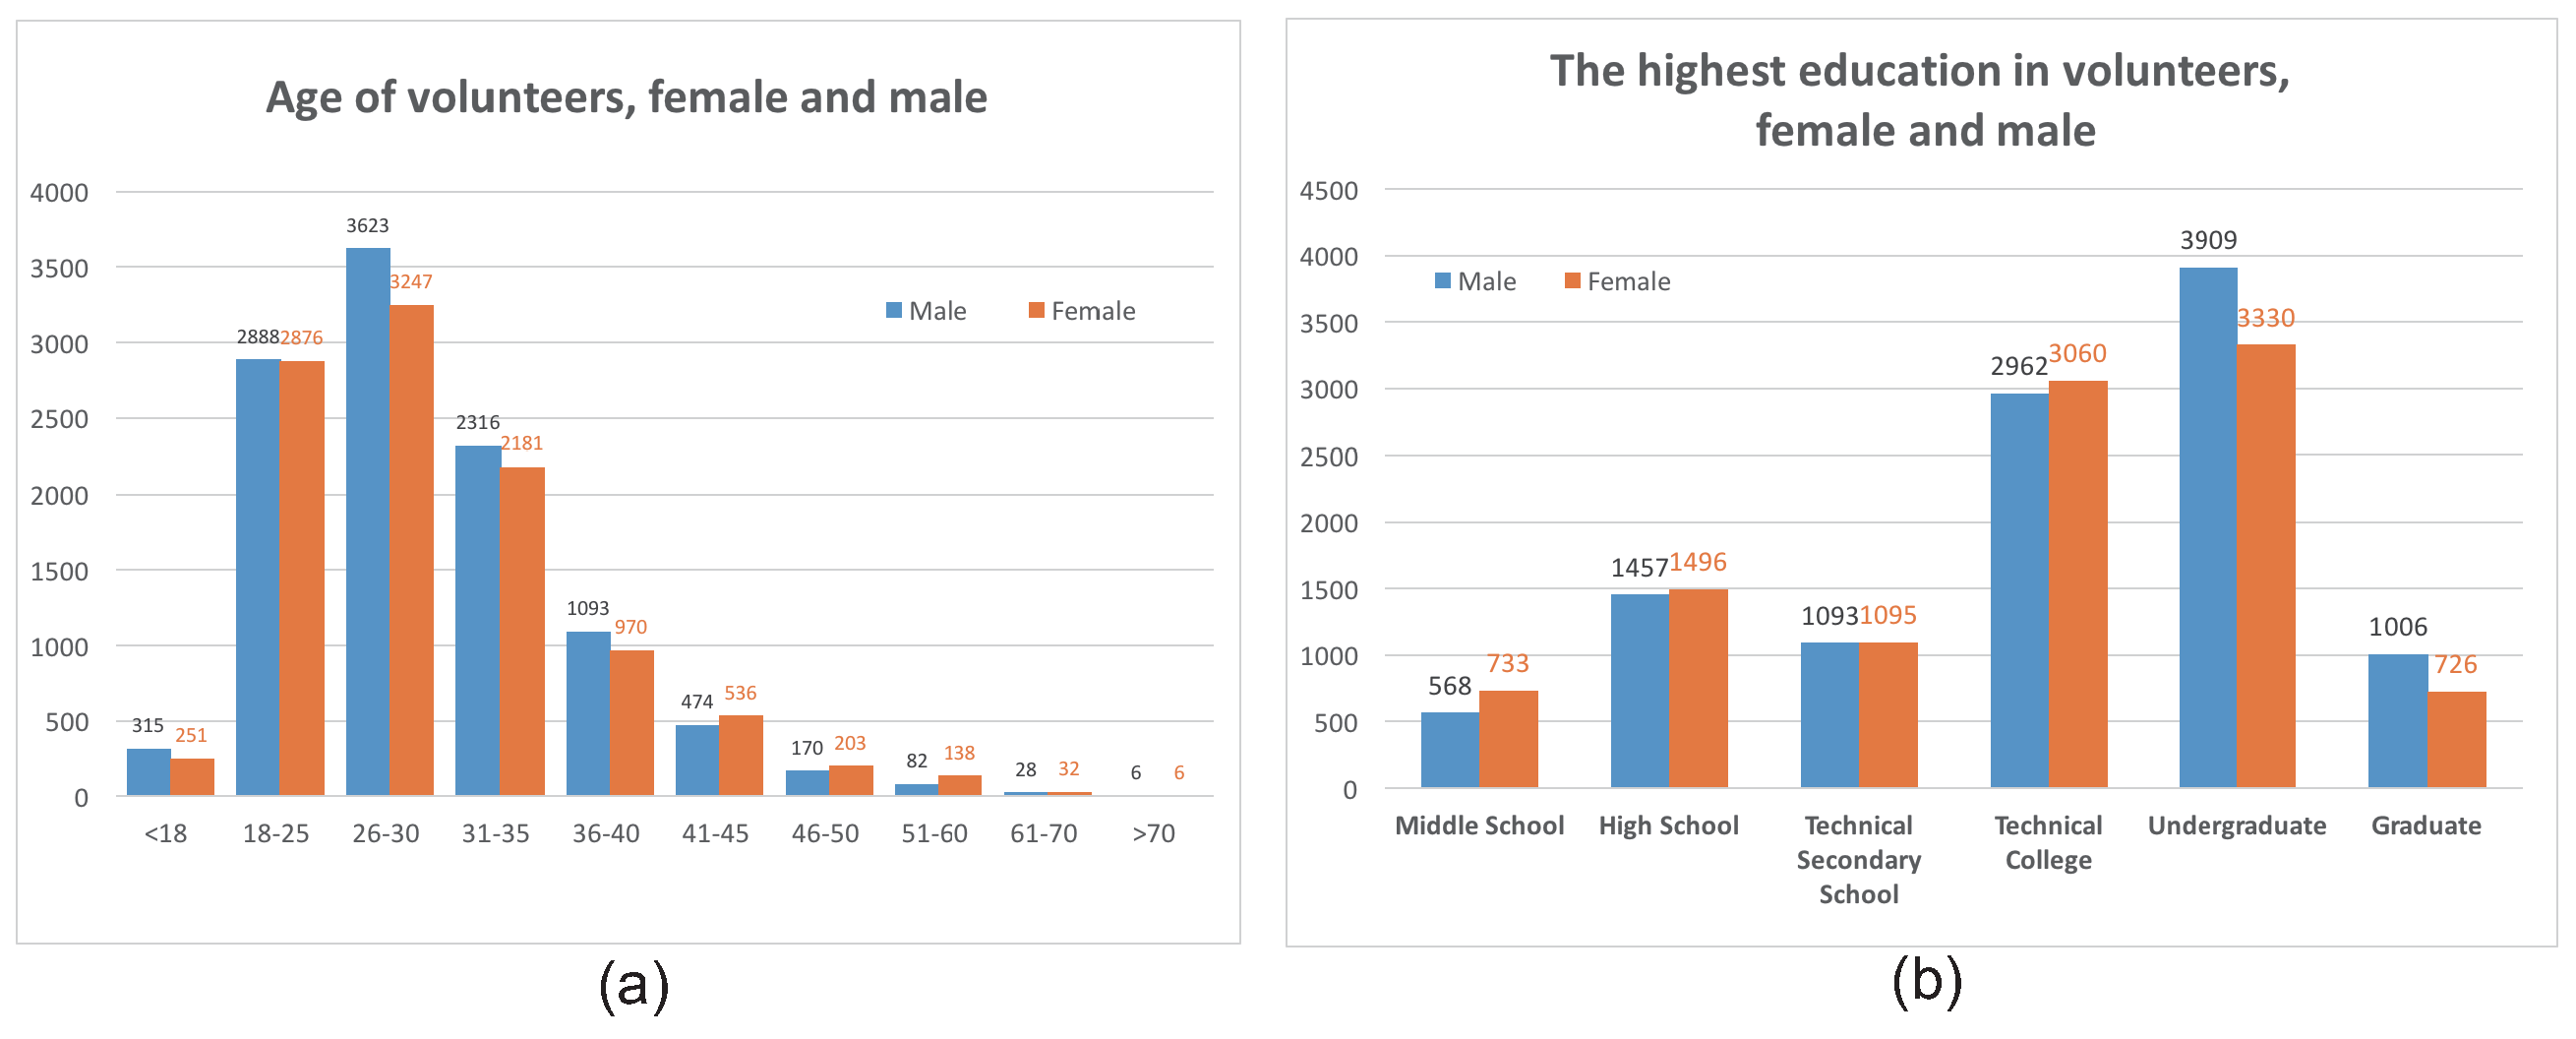
\includegraphics[width=\columnwidth]{pictures/data1}
 \caption{Age and Education Distribution: (a) age; (b) education}
 \label{fig:data_age_edu}
\end{figure}

Figure~\ref{fig:data_age_edu} gives the distribution of age and education over the population. It shows that samples cover a wide range of ages, dominating between 18 to 45. There is also a few records pertaining to individuals below the age of 18 or above 70. The distribution follows the fact that Shenzhen is a city where the majority is young people. According to the 2015 Annual Census Statistics report\footnote{http://www.sztj.gov.cn/xxgk/tjsj/pcgb/201606/t20160614\_3697000.htm}, people aging 15-64 occupy 83.23\% and the median age is 31.5. Figure~\ref{fig:data_age_edu} gives the distribution of education levels, ranging from low to high. The technical college and university dominate the samples at the 61\% occupancy rate.

\begin{figure}[htb!]
 \centering % avoid the use of \begin{center}...\end{center} and use \centering instead (more compact)
 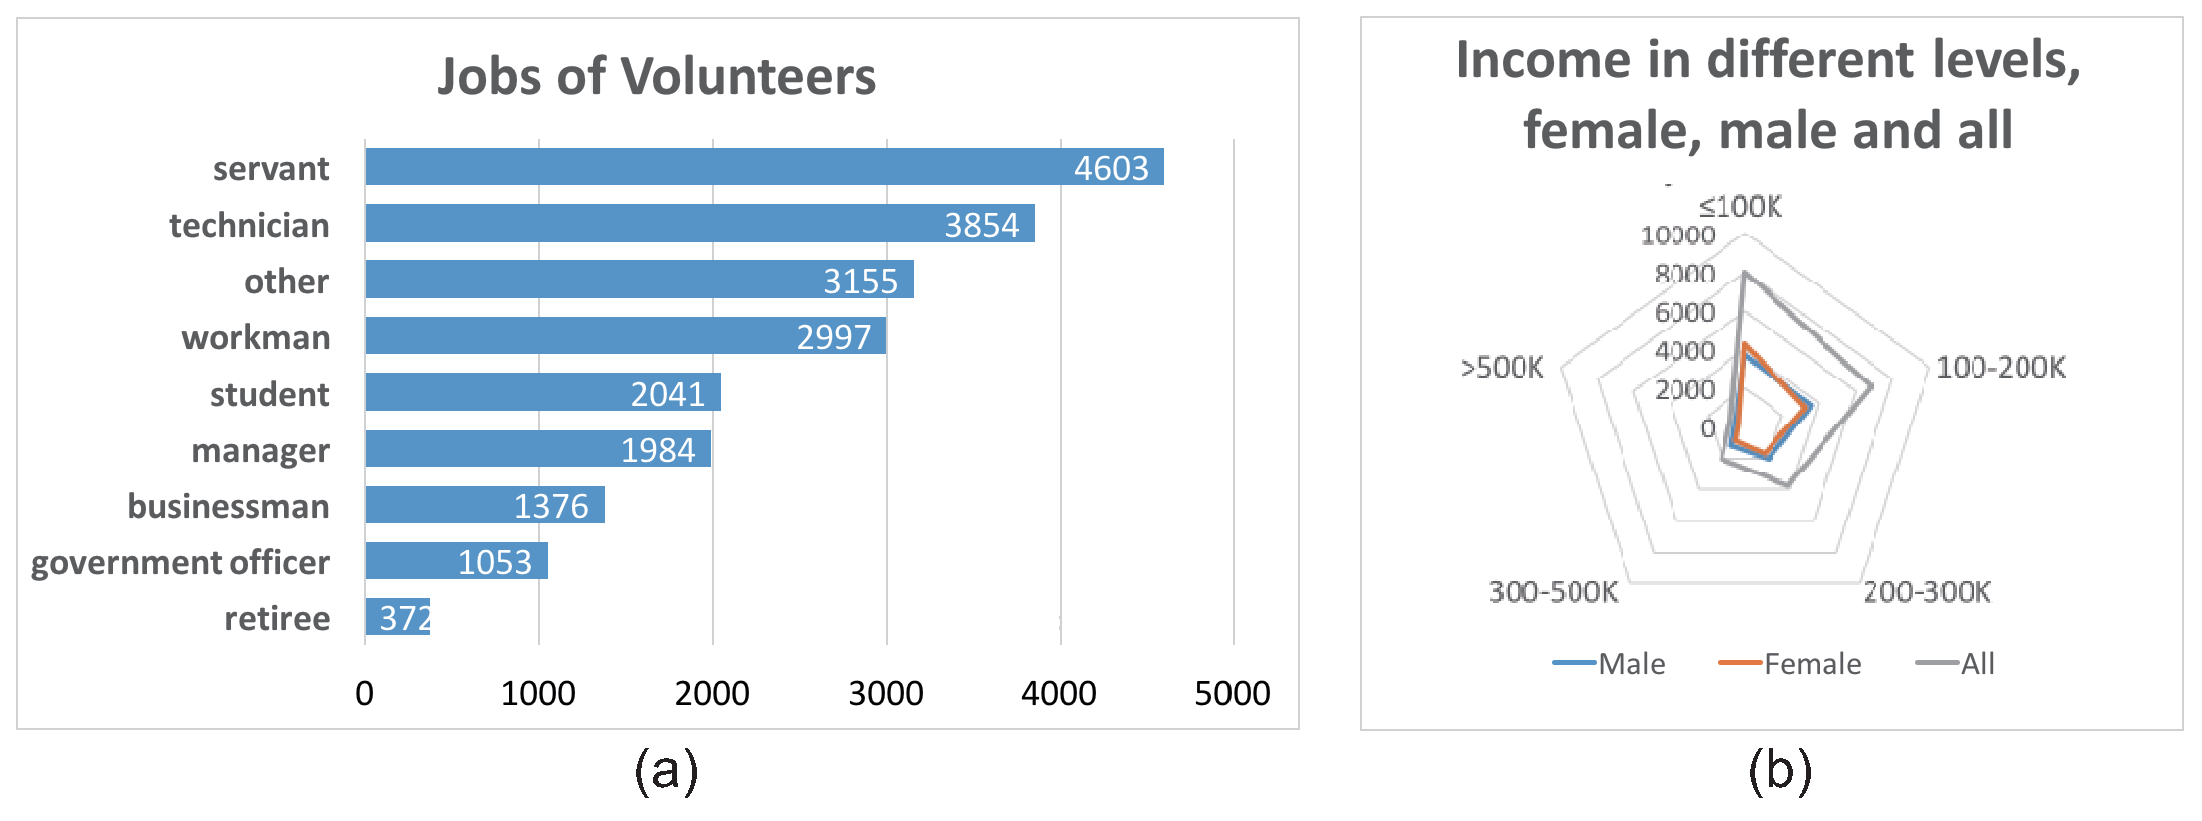
\includegraphics[width=\columnwidth]{pictures/data2}
 \caption{Job and Income Distribution: (a) job; (b) income}
 \label{fig:data_job_inc}
\end{figure}

Figure~\ref{fig:data_job_inc}(a) shows the job types of sampled individuals, who are servants, workers, officers, businessmen and so on. The covering of jobs is pretty wide. Figure~\ref{fig:data_job_inc}(b) gives the radar diagram of the annual pay. The majority get paid below 200 000. Individuals with higher salary are also reached in our census.

\begin{figure}[htb!]
 \centering % avoid the use of \begin{center}...\end{center} and use \centering instead (more compact)
 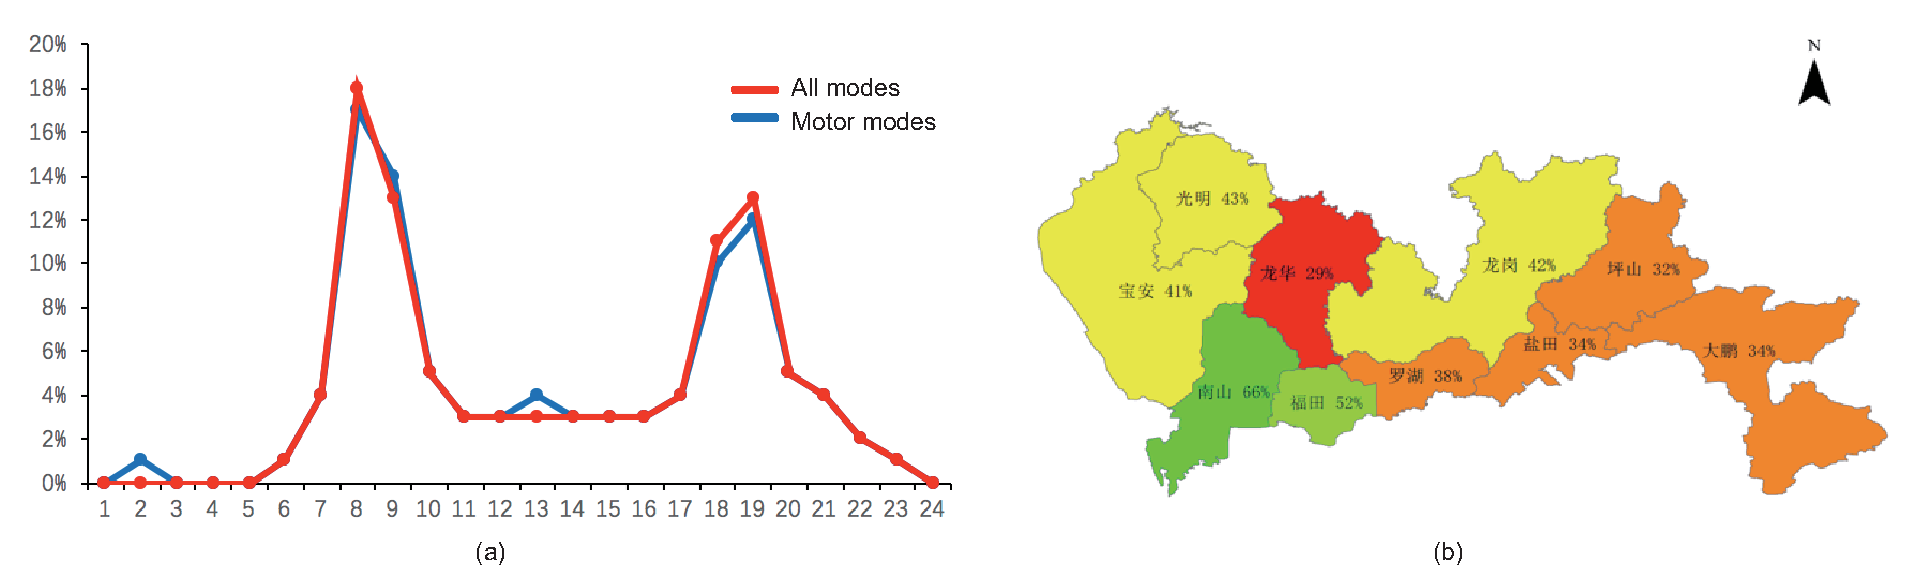
\includegraphics[width=\columnwidth]{pictures/data3}
 \caption{Statistics of Trips: (a) start time of trips; (b) purpose of trips; (c) distribution of origins/destinations }
 \label{fig:data_geometry}
\end{figure}

Figure~\ref{fig:data_geometry} shows the basic statistics related to trips. In Figure~\ref{fig:data_geometry}(a), the active traveling time (here, we take the start time as the representative of active time) follows the common knowledge of urban life. There are obvious morning and late afternoon peaks. Figure~\ref{fig:data_geometry}(b) gives the counting of different traveling purposes. 95\% trips are tagged with clear raveling purpose in the data. 33\% are going home and 37\% are going to work. Besides this kind of routine traveling, there are also substantial trips such as going shopping, going the hospital, etc. Figure~\ref{fig:data_geometry}(c) shows the spatial distribution of the origins and destinations. It is found that more dots are located in Futian and Nanshan districts, the city's heart than the surrounding areas. This is consistent to Batty's exposition of the focus of city networks and interaction patterns~\citep{batty2013new}.

% Trips are uploaded in a wide range of purpose in addition to home, work, but also includes XX entertainment, visiting, etc. The diverse purposes make it possible to characterize the flows across the city between different functional places.

Because there is always inevitable bias inherent in fully representing the ground truth of the population, the preliminary statistical analysis shows positive sign of a relatively even sampling of the population.


\section{Overview}
\wqc{Adding a background. Expert discussion. Summarize the tasks below.-0419}
\lmc{Add a paragraph to introduce the motivation of this work, where we derive the tasks via the interview with domain exports.-0420}

A discussion with experts in GIS. We summarize the analytic tasks identified from the interviews of domain experts. Then the workflow of the proposed visual analytics system.

\subsection{Goal}
\wqc{Common human mobility indicators: travel distance, travel time, travel frequency, radius of gyration and movement entropy. }\\

Spatial attractiveness is an important concept to evaluate ... in commercial activity, tourism and urban research. We interview the expert in GIS. \lm{They identify \textit{Spatial Attractiveness}, and their correlation with individual social characteristics as the core research concern. Furthermore, they want to explore the space diversity according to its attractiveness to individuals.} \lmc{I think first we introduce spatial attractivenss, which is well defined by previous work. Then we explain the diversity of lands in attractivess (we need to find a better term), which we define. I think it is ok.}

\begin{itemize}

  \item \textit{Magnitude of spatial attractiveness} How many persons could be attracted and how much the difficulty they overcome. \wqc{there is equation in related paper to support this.} \lmc{can you expand the spatial attractivenss, such as citing existing paper, explaining the concept, maybe with the equation is better.}

  \item \textit{Diversity of spatial attractiveness} Two types of diversity: diversity of the attracted persons, and diversity of attractiveness indicators. \wqc{cannot find this concept in papers, and, i am not sure about ``indicator"} \lmc{I defined this?}

\end{itemize}
With these questions, we summarize them into the tasks below, which need to be answered by our system.

\subsection{Tasks}
\lm{The exploration of core concepts above are resolved further with following tasks... to align the analysis of mobility patterns with individual characteristics. Before diving into the design of the system, introduce the couple of specifical tasks the system intended for.}

%The design of the system is driven by tasks, to align the analysis of mobility patterns with individual characteristics. Before diving into the design of the system, introduce the couple of specifical tasks the system intended for.

\begin{itemize}
\item \textit{Task 1: Identify the group with specific individual characteristics\wqc{What kind of citizens tend to be attracted?}}: to get groups of people with common or close attributes, to explore the correlation among individual characteristics.
\item \textit{Task 2: What is the correlation between space and citizens? (Spatial Attractiveness)} to understand... group of citizens are attracted to different places, e.g., to know the similarities and differences between different groups in their mobility patterns, to investigate the relationship between movement and individual characteristics.

\item \textit{Task 3: What is the detailed properties of attractive differences?} ... How many citizens are extracted, the origins (Where do the attracted citizens come from?) What is the attractive differences over groups? 

% City has different function areas. Some areas meet all the basic requirements of citizens' living activities, while some cannot. ... 

% \item \textit{Task 2: Why the attracted citizens are attracted?}: to explore ... \lmc{I don't think we can explain why...}
% \item \textit{Task 3: How many citizens are extracted?}: to express ... \lmc{I think it is just numbers, too weak to be a task}
% \item \textit{Task 4: Where do the attracted citizens come from?}: \lmc{also here}. City has different function areas. Some areas meet all the basic requirements of citizens' living activities, while some cannot. ... to know the similarities and differences between different groups in their mobility patterns, to investigate the relationship between movement and individual characteristics.
\end{itemize}

\subsection{Design Considerations}

With these three tasks, we derive following design considerations:

\begin{itemize}
\item \textit{Intuitive perception of an individual as an organic complex (C1)}: the system should make use of users' daily life experience in knowing people to provide intuitive visualization, instead of the lifeless representation by number. The visual design needs to help end-users to pick desirable ones from the mass.
\item \textit{Good overview of the multivariate individuals (C2)}: following the visual analytics manta by Shneiderman~\citep{RN459}, it is very important to provide a good overview of all the individuals then the users know where to explore.
\item \textit{Effective multivariable cross-filter for individual characteristics (C3)}: there are eight domains to describe an individual. The system is supposed to provide a straight-forward way for easy filtering by the eight criteria.
\item \textit{Compact visualization of mobility patterns in the constraint of spatial space (C4)}: the analysis of mobility patterns not only includes the conventional spatial and temporal dimensions, but also other abstract dimensions, e.g., travel purpose, visiting frequency, etc. The system should handle a compact layout to support the easy correlation between spatial and abstract information.
\item \textit{Flexible interactions to explore the mobility patterns either within one group or between groups (C5)}: to support the comparison among groups, \textit{Task 3}, the system should maintain flexible interactions which allow the end-users to explore freely.
\end{itemize}

% Classification method, flow clustering method, Semantic representation.

\iffalse
\begin{figure}[htb!]
 \centering % avoid the use of \begin{center}...\end{center} and use \centering instead (more compact)
 \includegraphics[width=\linewidth]{pictures/teaser.eps}
 \caption{System Interface: (a) an interactive infographics provides the basic statistic facets of individuals; (b) a t-SNE visualization gives an overview of individuals, where the similarity in high dimensional space is preserved in 2D space; (c) data-driven profiles support users with organic individual perception; (d) group of interested individuals can be saved; (e) movement of the chosen group is visualized and explored in 2.5D main view; (f) a dock is provided to restore and compare findings; (g) different choices of 2.5D encoding can be selected.}
 \label{fig:teaser}
\end{figure}
\fi

\begin{figure}[htb!]
 \centering % avoid the use of \begin{center}...\end{center} and use \centering instead (more compact)
 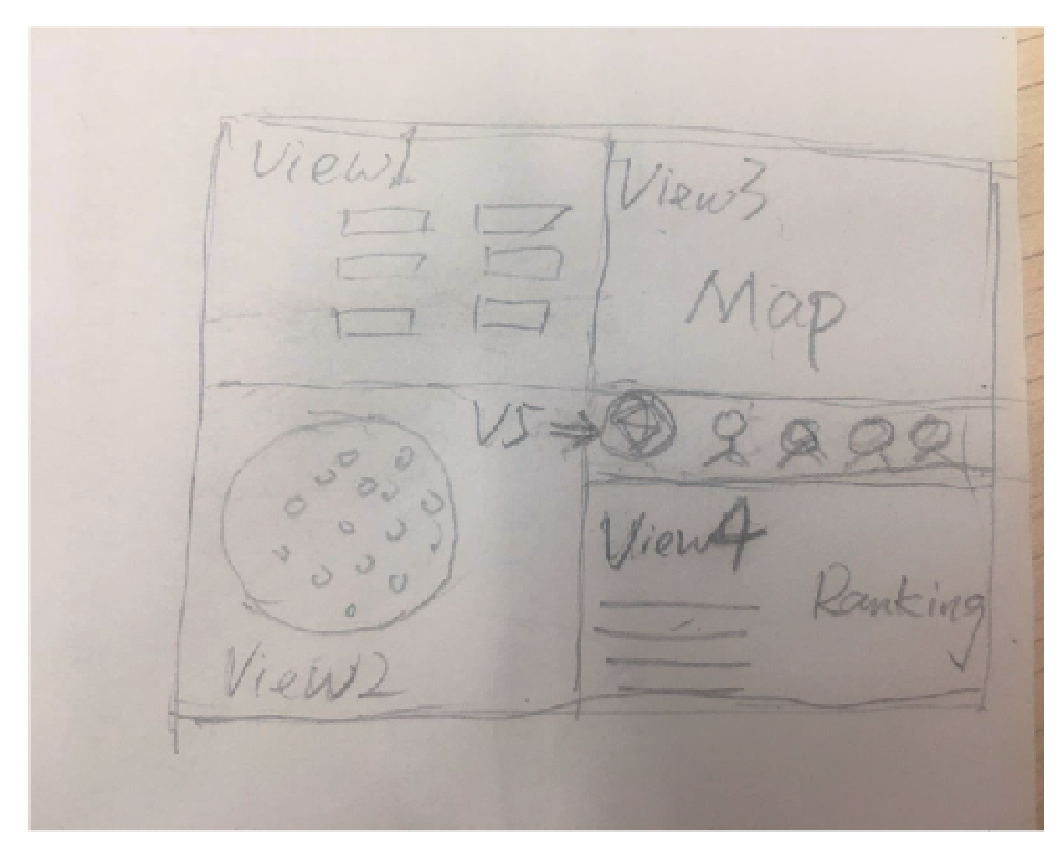
\includegraphics[width=\linewidth]{pictures/interfaceDraft.eps}
 \caption{\wq{System Interface: (a) an interactive infographics provides the basic statistic facets of individuals; (b) View1: a XXXX visualization gives an overview of individuals, where the similarity in high dimensional space is preserved in 2D space; (c) View2: data-driven profiles support users with organic individual perception; (d) View3: map view for movement of the chosen group; (e) View4: for ranking or comparison; (g) View5: top N kinds of citizens with social characteristics.}}
 \label{fig:interfaceDraft}
\end{figure}



\section{Visual Design}

With those design considerations (introduced in Section~\ref{}), we develop a visual analytics system as Figure~\ref{fig:interfaceDraft} shows. It composes of individual panel (the left part) for individuals (\textit{Task 1}) and spatial panel (the right part) for the mobility pattern (\textit{Task 2 and 3}). In the individual panel, interactive infographics, t-SNE visualization, and data-driven profiles support users to narrow the scope down to groups of individuals with interested characteristics. With the chosen group of individuals, its moving related information is visualized and explored in a 2.5D spatio-temporal view. \lmc{Show a overview figure, to introduce the relationship between multiple views}


% overview of the data. Encode information but also allow users to set multiple criteria (\textit{C1}). Support users to slice the data by different domains.}
% Semantic understanding of social characteristics.


\subsection{Data-driven Profile Visualization}

Glyph-based visualization~\cite{borgo2013glyph} is the form of visual design to compose multivariable into a collection of unified visual symbols, known as a glyph. A glyph is intended for quick understanding and aligned comparison. \lm{Dual glyphs are designed, to illustrate the information of individual from two different perspectives, i.e., detailed inspection of individuals and efficient comparsion over multiple individuals.}

\paragraph{Star-like Glyph} \lm{To compare over multiple individuals, a star-like glyph is designed to summary each individual, to ease the comparison by common coordination configurations....}


\paragraph{Cartoon Glyph} ... Among glyph design, Chernoff Face~\cite{chernoff1973use} represents data variables by the different features of a cartoon face. Following the idea of Chernoff Face, we design a type of glyph, a graphical representation of people with specific individual characteristics. The idea behind using faces is that humans easily recognize faces and notice small changes without difficulty (\textit{C1}). Those visual profiles are intended for intuitive visual understanding, from abstract to concrete and semantic understanding, to support users to target the interested individual groups effectively.

Figure~\ref{fig:design_profile} shows the legend for the user profile. The eight domains are encoded by visual symbols and organically organized in a human figure. There are basically three types of variables to drive the figure, i.e., the numeric, categorical and boolean ones. For numeric attributes such as income and education levels, visual symbol keeps consistent design but with changing visual variation, such as size, thickness. For the categorical attributes such as job, visual symbols are designed separately for better semantic meaning. For the boolean attribute like car, house, a symbol is designed to indicate its existence. With this consideration, the domains are designed as follows:

\begin{figure}[htb!]
 \centering % avoid the use of \begin{center}...\end{center} and use \centering instead (more compact)
 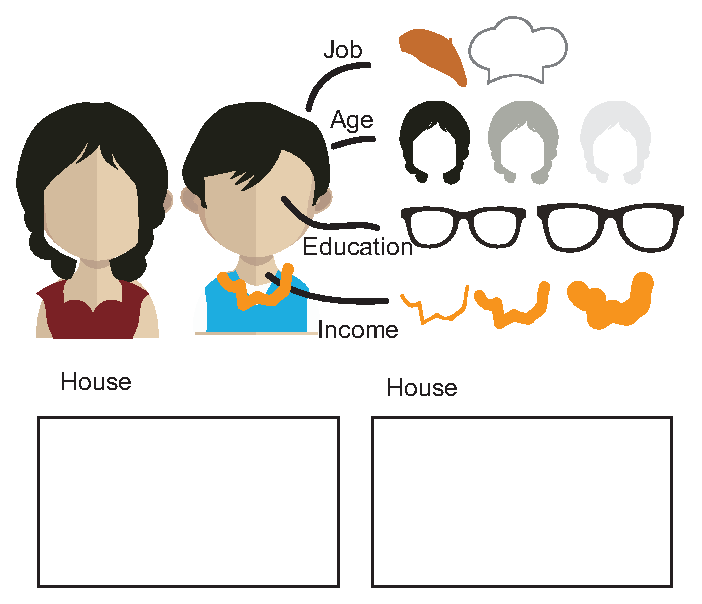
\includegraphics[width=\columnwidth]{pictures/design_profile}
 \caption{Design Profile: the eight characteritical domains are encoded and organized in an organic human figure.}
 \label{fig:design_profile}
\end{figure}

% For numeric attributes.

% By different composition, stimulus pattern which has the abstract demographic measurement of individuals.

\begin{itemize}
\item \textbf{Gender} the gender is visually mapped to the hairstyle of the avatar.
\item \textbf{Age} age is implied by the decoration on the hair. For the elder above 70, the hair is dyed to gray. For the youth beneath 18, a hair decoration is adapted for the different hairstyles of girls and boys.
\item \textbf{Education} The thickness of eyeglasses is used to indicate the different levels of education.
\item \textbf{Job} The clothes is designed to imply the job of the individual. There are 9 types of clothes.
\item \textbf{Belongings} for real estate, car, residential license are considered as the belongings to the individual, so we design each of them as an add-on decoration to imply whether the individual has it or not.
\item \textbf{Income} a money symbol is used to represent the income, whose size encodes the income level. The more money an individual earns, the larger the symbol is.
\end{itemize}

\begin{figure}[htb!]
 \centering % avoid the use of \begin{center}...\end{center} and use \centering instead (more compact)
 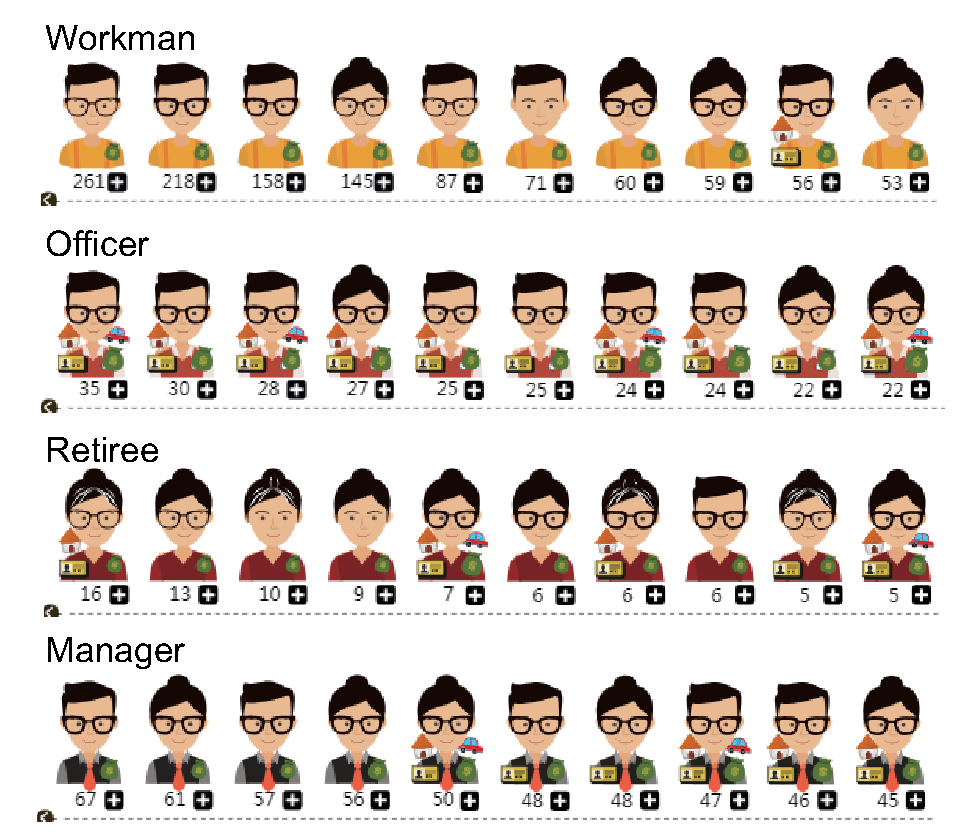
\includegraphics[width=0.6\columnwidth]{pictures/design_example}
 \caption{Representative figures with the top 10 largest population in four jobs}
 \label{fig:div_example}
\end{figure}

With the visual mapping, the profile varies from individual to individual. By concretizing the attributes which otherwise is too abstract to percept, users can scan and search for interesting target effectively. Figure~\ref{fig:div_example} lists the figures with the top 10 largest population in some job. The textual number beneath indicates the population. It is found that the majority of workmen earn a low salary and most of them have no residential license. On the contrary, for the officers, all of them have the residential license and most of them have a house. Some of the retired people are in old age. Most of the managers are at undergraduates, even graduates.


\wq{\subsection{XXXX Projection of Individuals}}
\wqc{A octagon radar graph to position all citizens. A clustering algorithm for commend similar persons into a new group.(maybe: interactions to set the weight of each characteristic)} \lmc{Yes, I think an interactive weight adjustment is good.}

\begin{figure}[htb!]
 \centering % avoid the use of \begin{center}...\end{center} and use \centering instead (more compact)
 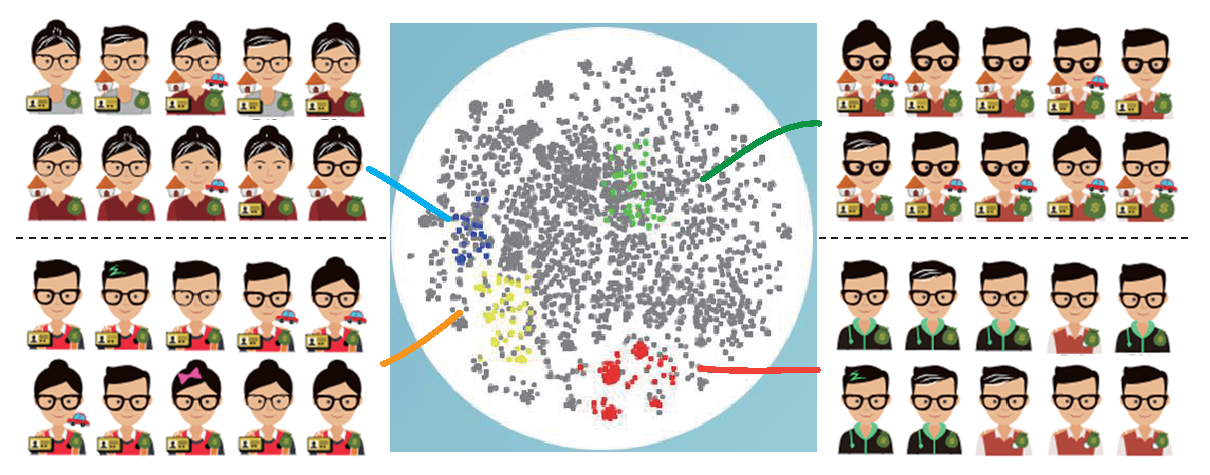
\includegraphics[width=\columnwidth]{pictures/tsne}
 \caption{t-SNE project with four groups of the interest: (a) t-SNE project }
 \label{fig:tsne}
\end{figure}

In our case, each individual can be denoted as a vector $x_i$ with eight factors, and we get high dimensional data set $X={x_1, x_2, ..., x_n}$. The dimensionality reduction techniques are to preserve the local structure of high dimensional data in low dimensional space, which are efficient approaches to provide a good overview of the multivarible individuals (\textit{C2}). We adapt t-SNE project~\citep{maaten2008visualizing} to project $X$ as two-dimensional dots $Y={y_1, y_2, ..., y_n}$. One of steps in t-SNE is to compute the conditional probabilities to represent the similarity based on the distance between high dimenional datapoints. The conditional probability $p_{j\mid i}$ between $x_j$ and $x_i$ is given by:

\begin{equation}
p_{j\mid i} = \frac{exp({\left \| x_i - x_j \right \|}^2/2\alpha_i ^{2})}{\sum _{k\neq i}exp({\left \| x_i - x_k \right \|}^2/2\alpha_i ^{2})}
\end{equation}

where $\alpha_i$ is the variance of the Gaussian that is centered on $x_i$. Specifically in our context, the high-dimensional Euclidean distances $\left \| x_i - x_j \right \|$ between $x_i$ and $x_j$ needs to be adpated the numerical and categorical characteristics. Characteristics such as age, income, are numerical and comparable, so the difference exactly explains when they are different. But the other characteristics, i.e. job, real estate, car, residential, are ordinal. There is not the numeric order. For example, the job distance from a manager to a businessman and a workman is not comparable, which is considered the same distance, i.e., set to 1.


As Figure~\ref{fig:tsne}shows, all 21435 volunteers are embedded in the 2D view, where the closer two dots are, the more similar they are in the eight characteristics. Figure~\ref{fig:tsne} exemplifies four features groups of dots in a neighbor.

Multiple views of abstract view, t-SNE protection, and semantic data-driven profile visualization are coordinated in a Cross-filter machinesm~\citep{Weaver2010}. It allows end-users to interactive drill-down into individuals with interested characteristics from multiple perspectives(\textit{C3}). Starting from the abstract criterion constraints, the scope of interest is narrowed down to individuals with(out) certain characteristics. And then further cross-filtering with semantically visual profiles can be performed to check the combination of 8 characteristical variables.

\iffalse
\subsection{2.5D Spatial Visualization}
\label{subsec:25D}

\begin{figure}[htb!]
\centering
\subfigure[]{
\resizebox*{9cm}{!}{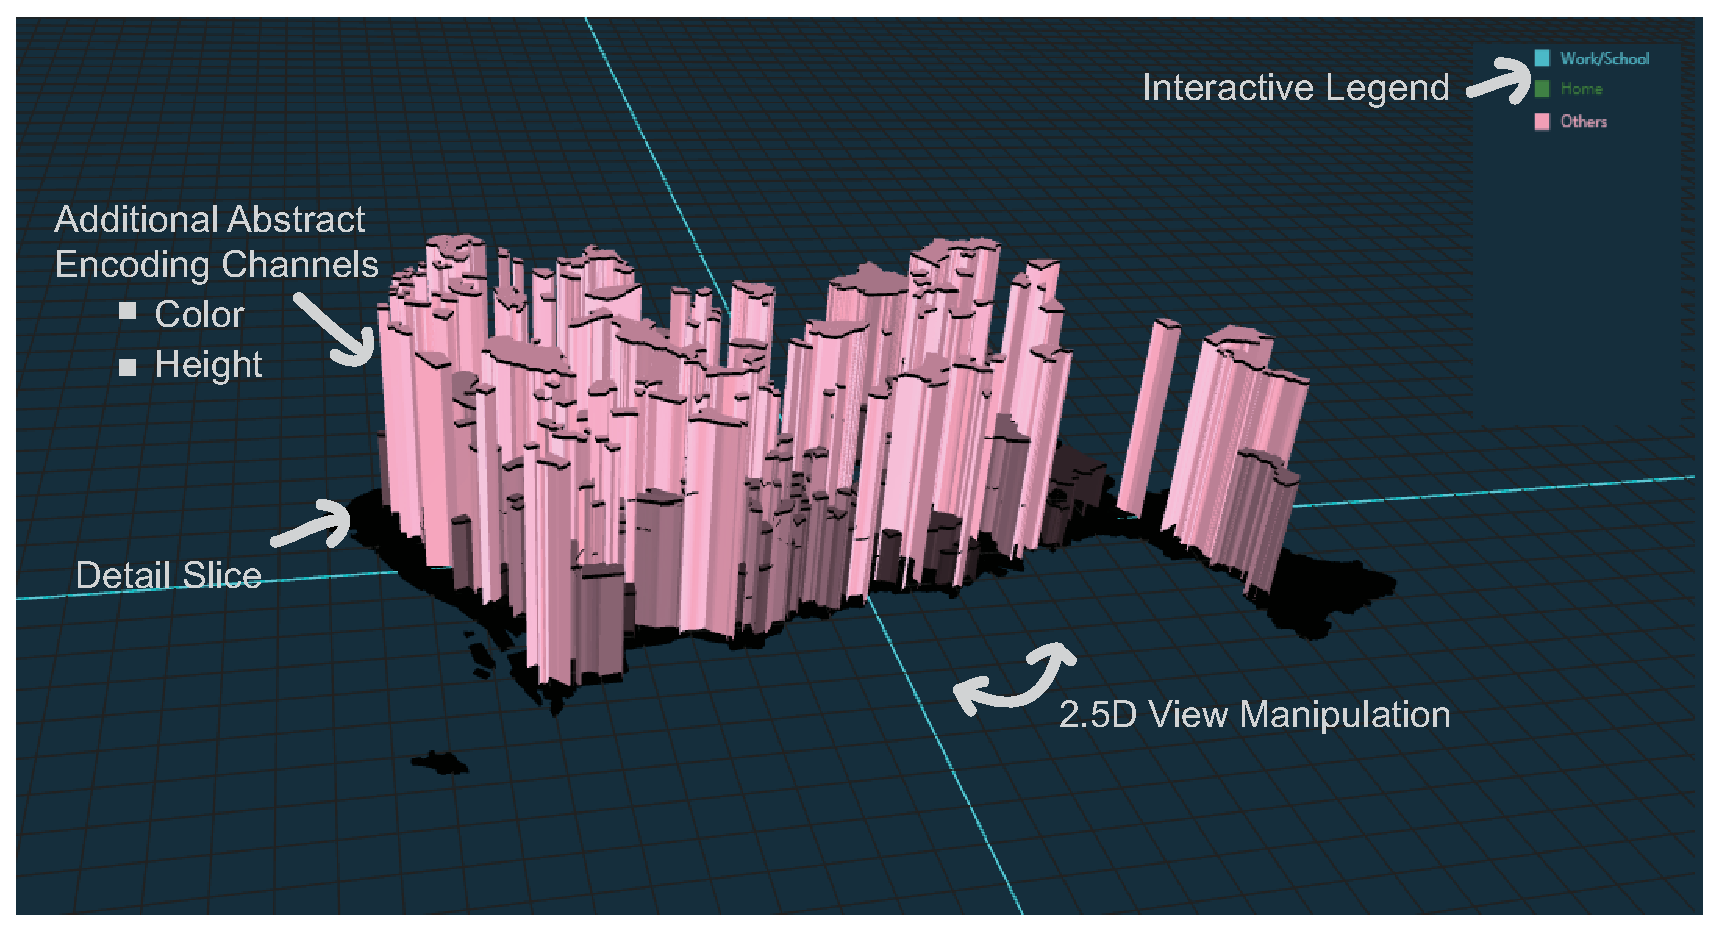
\includegraphics{pictures/space1.eps}}}\hspace{5pt}
\subfigure[]{
\resizebox*{9cm}{!}{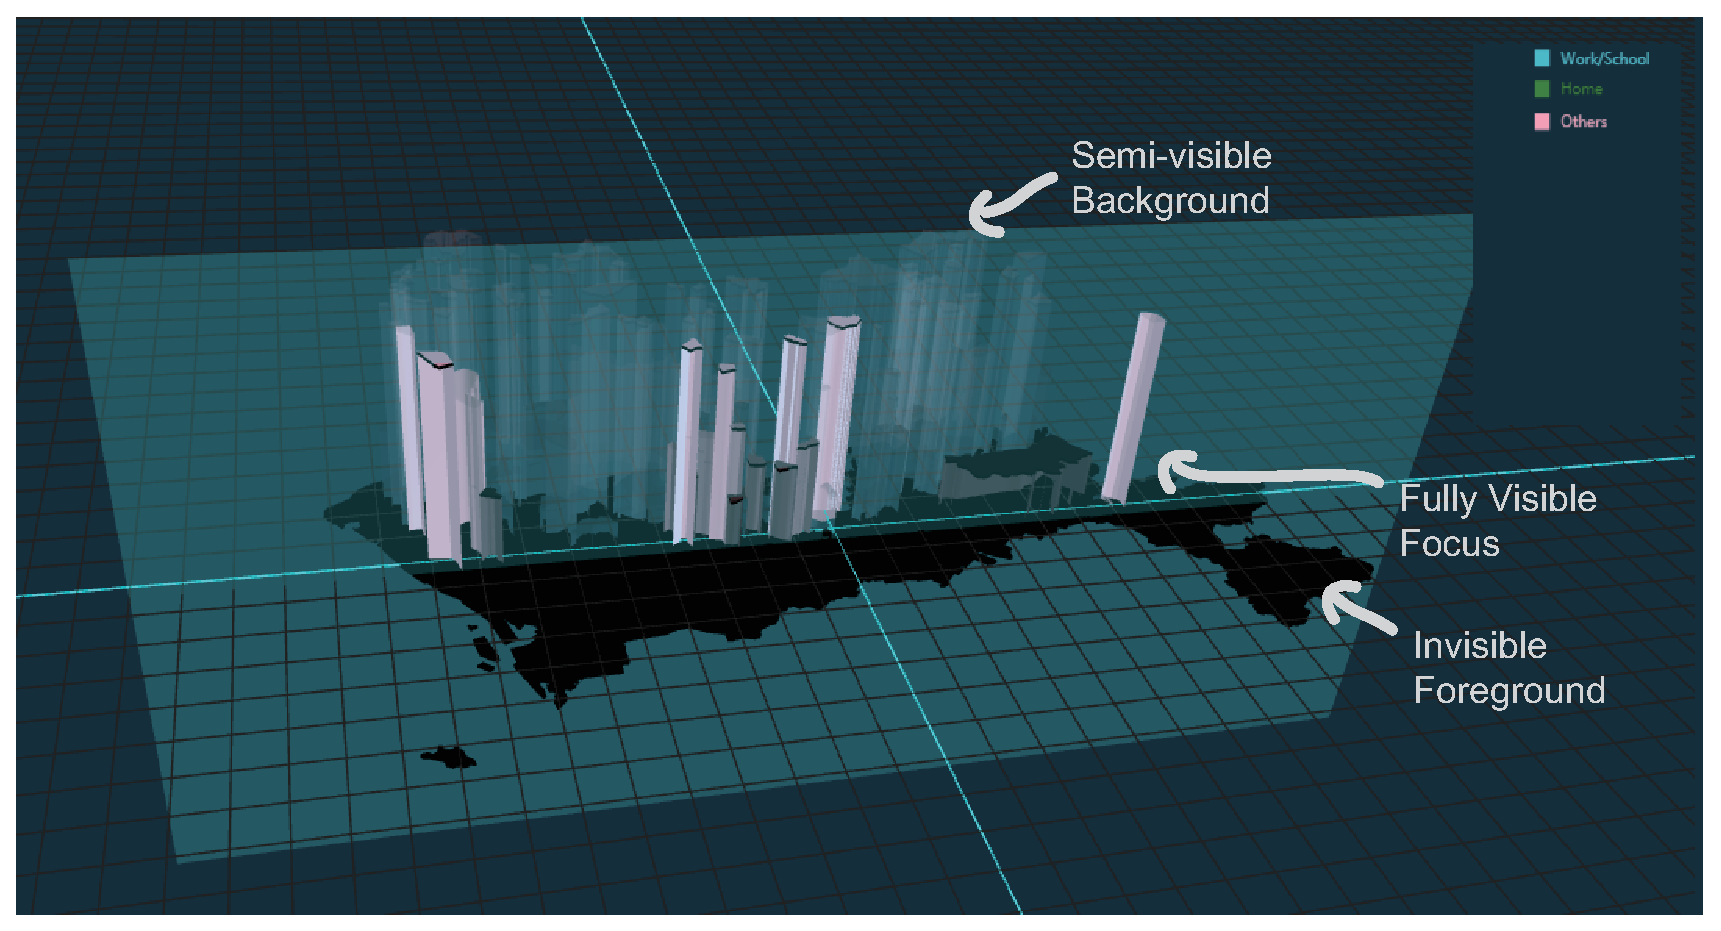
\includegraphics{pictures/space2.eps}}}\hspace{5pt}
\caption{2.5D Spatial Visualization: (a) 2.5D spatial visualization with z-axis to encode addition information; (b) detail slicing in 2.5D space.}
\label{fig:2.5D}
\end{figure}


Embedding multiple variables in the spatial map is a challenging problem. Distorting 2D spatial for better space usage, such as the partial route embedding~\citep{sun2016embedding} is an effective method when there are a few local foci. When it comes to the global visualization, there is always a trade-off between occlusion-free and the compact spatial perception. Following the idea of stacking 2.5D space design~\citep{Tominski2012_stacking}, the space in this work is embedded in 2.5D space, to relax the z-axis for additional abstract information encoding.

Figure~\ref{fig:2.5D}(a) shows the 2.5D visualization. The spatial map consists of Traffic Analysis Zone (TAZ), which is the unit of geography holding a certain number of people. For the 2.5D, each TAZ is grown as a prism whose height and color are developed to encode abstract information, e.g., the occurrence of visiting. With difference encoding choices, it is capable to visualize the correlation between spatial and different attributes (\textit{C4}). For example, in Figure~\ref{fig:2.5D}(a), prisms' height and color both encode the ratio of none-routine trips (such as go entertainment, go hospital, etc.) in the whole. For better 3D visual perception, lighting is turned on. Also, a lid is laid on the top of each prism to clearly bound its extent at the z-axis.

Several interactions are integrated into the spatial view to alleviating the occlusion problem (\textit{C5}). The manipulation of 2.5D view supports users with rotate, zoom, pan operations, which are so continuously flexible that users probably find a suitable observing point. In the cases where occlusion is inevitable, an interaction named as \textit{Detail Slicing} is developed, as Figure~\ref{fig:2.5D}(b) shows. Detail Slicing is the operation to put a cross-section in the 2.5D space to expose the TAZ inside. To contextualize the cross-section, TAZs are visually adapted according to the intersection by ray casting. The TAZ in the foreground will be hidden, the intersected TAZs will be fully visualized and the ones in the background will be in semi-transparency.


To compare the mobility patterns across different groups of people, a Small Multiple dock is used to reserve the ever explored interesting result (Figure~\ref{fig:teaser}(f)). To simply the comparison over spatial distribution, the snapshot is also rendered in the 2.5D space, which maintains the same interactions as the main 2.5D space does.
\fi



\wq{\subsection{A glyph design to show travel indicator (in view3, in case1)}
We design a kind of glyph to express a high-dimensional travel indicators. It will be embeded in the map view\wqc{for case1}. \lmc{This is great! more indicators, the better. }
The elements may be included in the glyph:
\begin{itemize}
  \item (home-work distance)
  \item travel distance
  \item travel radius
  \item travel frequency
\end{itemize}}


\wq{\subsection{A glyph design to show attractiveness (in view3, in case2)}
We design a kind of glyph to express spatial attractiveness.
The elements may be included in the glyph: \lmc{We can explain each of the indicator a bit. But do it later after the implementation.}
\begin{itemize}
  \item quantity
  \item distance
\end{itemize}}

\wq{\subsection{A glyph design to show attractiveness diversity(in view3, in case3)}
We design a kind of glyph to express spatial attractiveness.
The elements may be included in the glyph: \lmc{we need to find terms similar to above}
\begin{itemize}
  \item \lm{Purpose Number} how many kinds of purpose?
  \item  the percentage of each purpose?
\end{itemize}

(if comparison between groups, the glyph up, show the diversity of multiple groups at the same time.)}


\section{Experts Feedback}

\lmc{Add a section to introduce the domain experts' feedback}

\lm{We interview XX domain experts from the GIS field. XX of them are with ... The procedure went as following. We first introduce them the system an...}

\section{Case study}

In this section, we apply the method described above to study the case of Shenzhen. We introduce the several cases to demonstrate the usage and effectiveness of the system.


\wq{\subsection{Case 1: find diversity of citizens based on social characteristics}}
\wqc{Aim1: use view1 and view2 for groups. Aim2: show their basic activity spaces in view3 and view4. text no changes yet.}

This work is inspired and motivated by the implication in science fiction~\textit{Folding Beijing}, which is that people are categorized into three classes and behave in the parallel spatial-temporal patterns. The first cast explores whether the folding city exists in reality or not.

\begin{figure}[htb!]
 \centering
 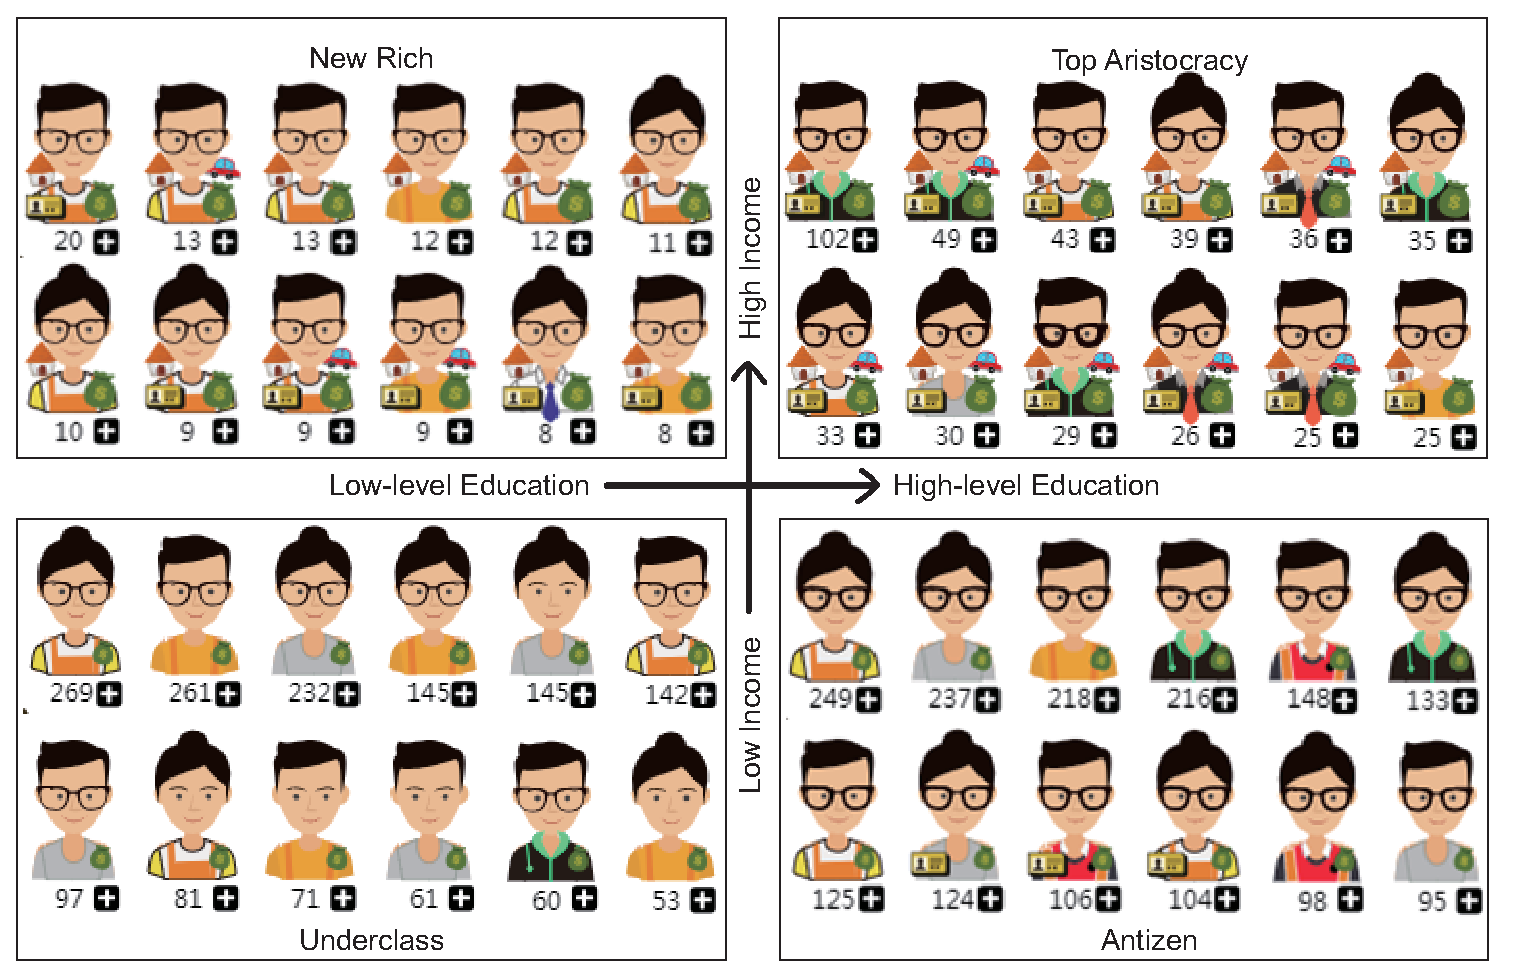
\includegraphics[width=\columnwidth]{pictures/case1_1}
 \caption{Four Groups Divided by Income and Education Characteristics}
 \label{case11}
\end{figure}

Although it is incomplete, income and education are two of the most essential characteristics to tag an individual with a good resource or not.\\
\wq{EDIT paragraph below. not just give number, use view1 and view2 to filter the target groups.}\\
As Figure~\ref{case11} shows, taking income and education as the two dimensions, taking 300K yuan as the border between high and low income and an undergraduate bachelor degree as the border between high and low education level, four different groups are generated in the four quadrants. In the first quadrant, individuals are rich and well educated, who are in a group of so-called \textit{top aristocracy}. The second quadrant holds the group of \textit{new rich}, i.e., individuals with high income but low education income. In the third quadrant, they are the \textit{underclass} who has both low income and education level. The fourth quadrant is \textit{Antizen}, which is a new word to describe people have a good education but earn little.


Figure~\ref{case11} shows the top 12 profiles with the maximum population in each group. In each group, other characteristics surprisingly demonstrate the high correlation to income and education. For example, almost all of the \textit{top aristocracy} is with the residential license,  house, and car. On the contrary, \textit{underclass} do not have the residential license residence, neither the house nor the car. Most of \textit{New rich} has a house and work in the service industry.

Before diving into the complex mobility pattern analysis, we explore the home distribution of the four groups. As Figure~\ref{case1draft} shows, \textit{top aristocracy} and most of \textit{new rich} live concentrated in the downtown area of Shenzhen, where the living cost is higher, especially the housing cost. A small part of \textit{new rich} lives far away from the downtown, maybe because they don't have to work in downtown. The \textit{underclass} distribute more dispersively all over the whole city. Compared to the rich, they prefer the outer space because of the lower living cost. Lots of \textit{antizen} live in Nanshan District, where there are many universities and high-tech industrial parks full of well educated people.

\wq{The glyphs on the map means the travel distance, travel radius..., which is an important in mobility research. Describe the difference.}\\
\wqc{the 3rd design in Section.design, a kind of glyph for high-dimensional mobility indicator.}

\begin{figure}[htb!]
 \centering % avoid the use of \begin{center}...\end{center} and use \centering instead (more compact)
 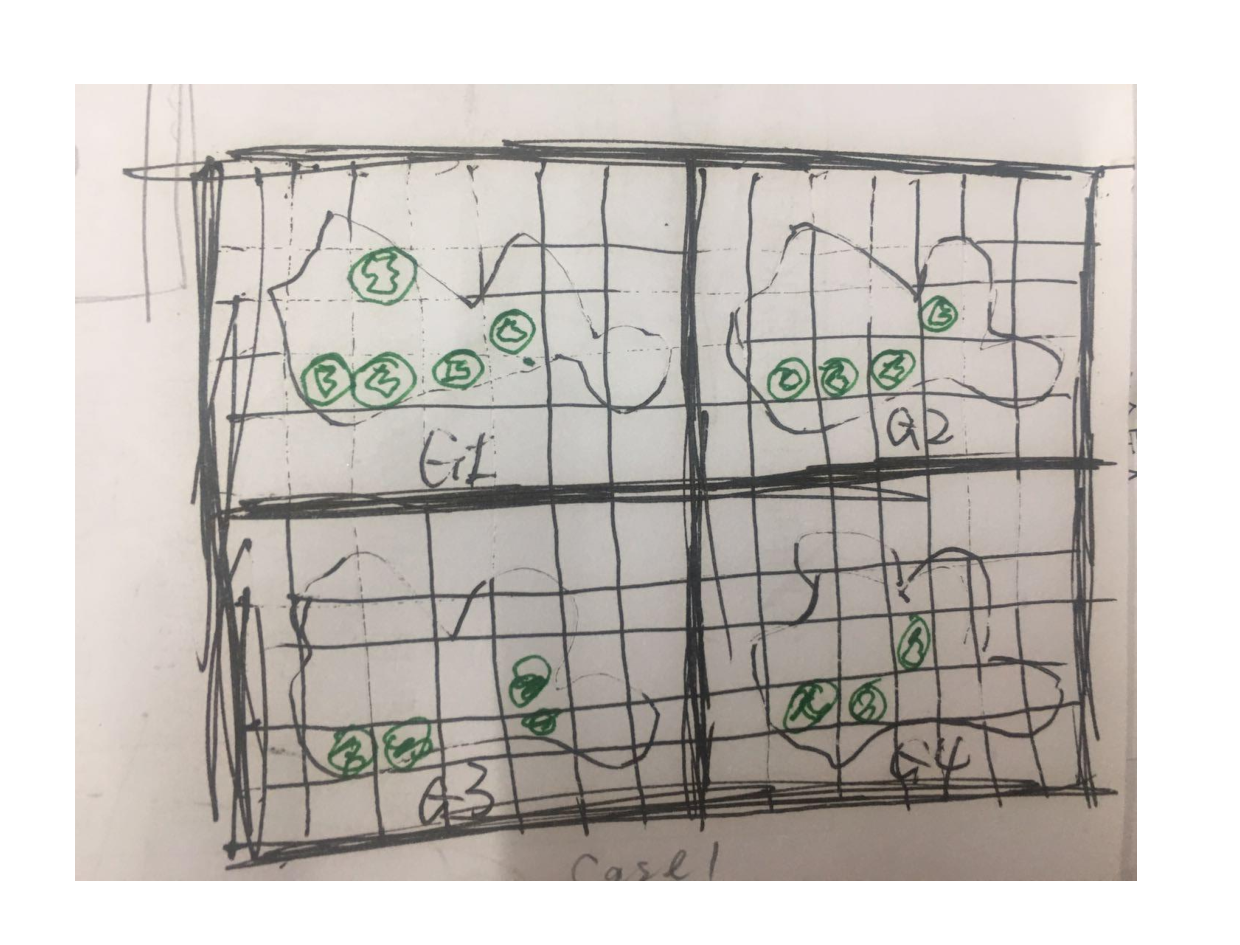
\includegraphics[width=\columnwidth]{pictures/case1draft}
 \caption{Home Distributions of the Four Groups}
 \label{case1draft}
\end{figure}

\iffalse
\begin{figure}[htb!]
 \centering % avoid the use of \begin{center}...\end{center} and use \centering instead (more compact)
 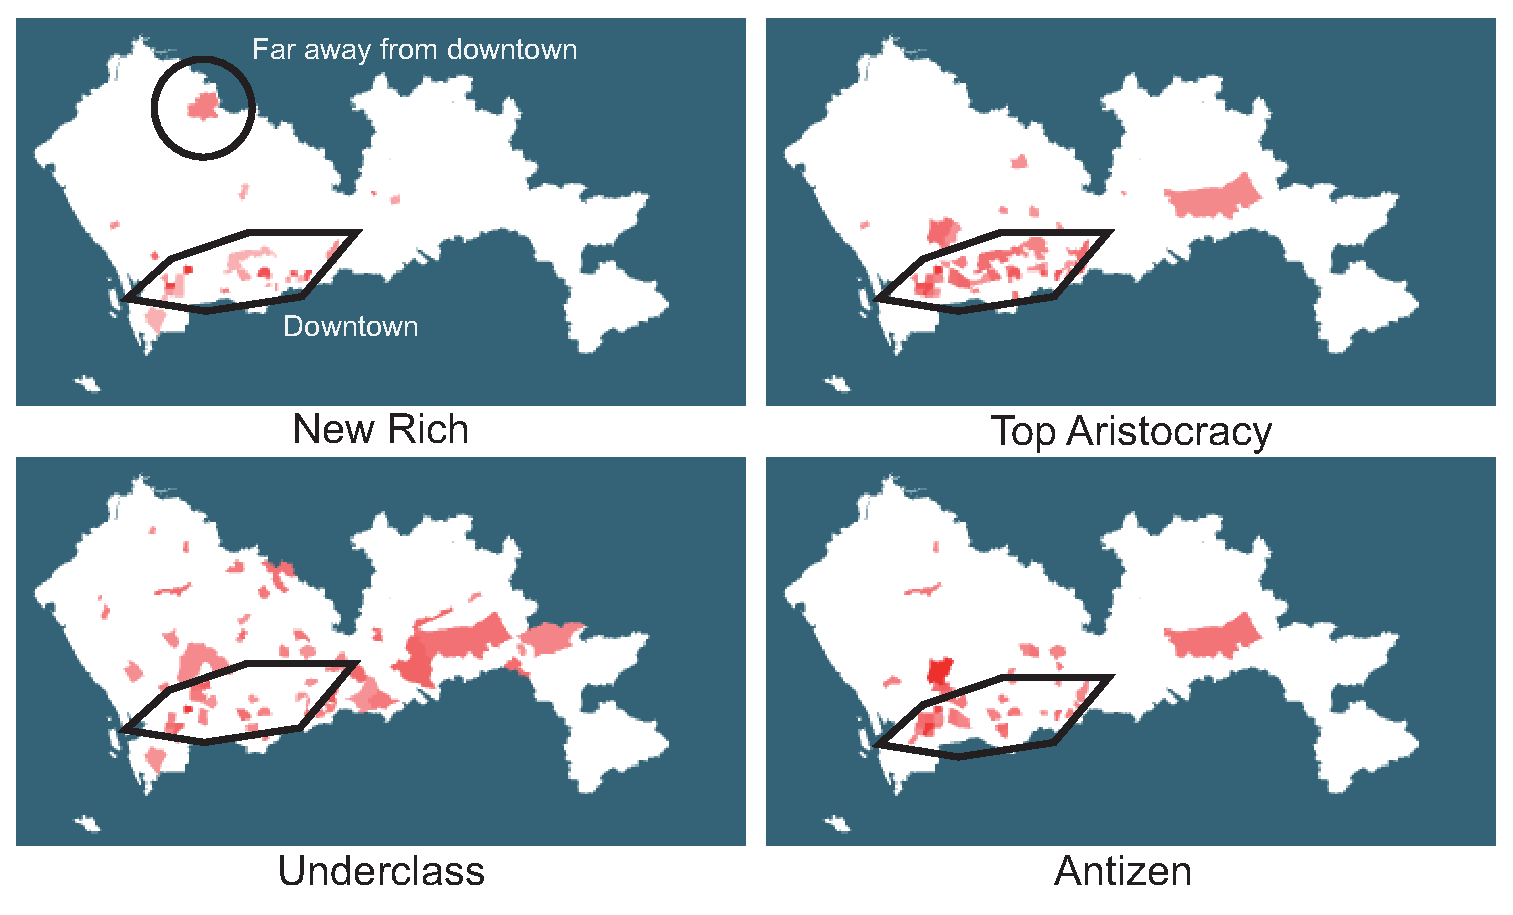
\includegraphics[width=\columnwidth]{pictures/case1_2}
 \caption{Home Distributions of the Four Groups}
 \label{case12}
\end{figure}

To have a better knowledge of mobility patterns of the four groups, trips are categorized into three categories, ``home", ``work'' for regular trips with the purpose of going home, work (or school for students), ``other'' for irregular trips with the purpose of shopping, visiting friends. Figure~\ref{case13}(a) shows the 2.5D overview of the three kinds of traveling categories. Each TAZ is grown to the same height, i.e., the unit one, and the height proportion of each traveling categories encodes the percentage of certain purpose in the whole, pink for ``others'', blue for ``work'' and green for ``home''. Although inside TAZ prisms are blocked in the Figure~\ref{case13}, our attention is drawn to the lifestyle of \textit{New Rich}. It is founded that the \textit{New Rich} travel for ``other'' purpose a lot, compared to other groups. To explore further, the detail slicing (introduced in Section~\ref{subsec:25D}) is applied to the four groups. Figure~\ref{case13}(b) shows three slices. It can be seen that individuals with low income (\textit{underclass} and \textit{antizen}) spend relatively more time on work, especially the \textit{underclass}. Working percentage is very small in-group \textit{new rich}. They live a more diverse lifestyle because they do many other things (the pink ones) except working.


\begin{figure}[htb!]
 \centering % avoid the use of \begin{center}...\end{center} and use \centering instead (more compact)
 \includegraphics[width=\columnwidth]{pictures/case1_3}
 \caption{Mobility Patterns of ``work", ``home" and ``not essential" of the Four Groups: (a) the overview of the three pecentage; (b) three slices for detailed comparison.}
 \label{case13}
\end{figure}
\fi



\subsection{Case 2: Diversity of spatial attractiveness of indicators}
\wqc{aim: with mixed purposes, show attractiveness quantity and entropy. View3 shows spatial attractiveness, including: quantity, distance, (direction); View4 shows ranking of origins, (or others); (add a interaction in view5 for citizens in selected grid.)}

\wq{Due to the various functions of the areas, for different space, the attractiveness indicators differs. Therefore, in this case, we demonstrate the use of the system for exploring diversity of spatial attractiveness indicators. }

\wq{As Figure~\ref{case2draft} shows, in view3, glyph represents $\textbf{the quantity}$ and $\textbf{value of mixture of purposes}$. \wqc{(if we decide to give a computing equation to define it.)}\lmc{I think we can define a equation to compute it.} in view 4, ranking of each grid based on the quantity of each purpose.}
\begin{figure}[htb!]
 \centering % avoid the use of \begin{center}...\end{center} and use \centering instead (more compact)
 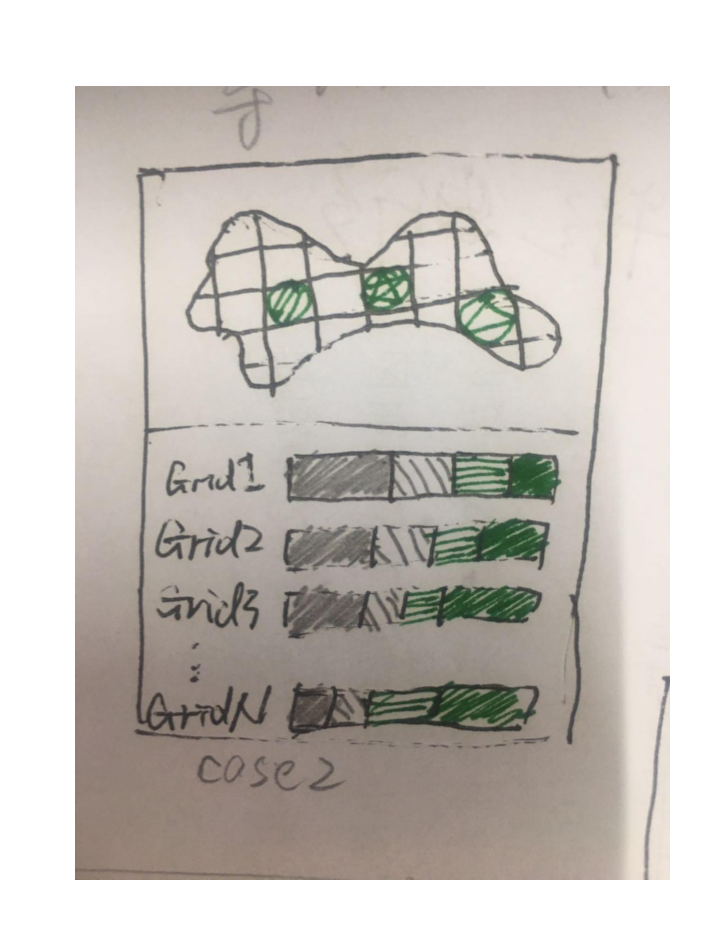
\includegraphics[width=\columnwidth]{pictures/case2draft}
 \caption{Trip purposes distribution of four groups with different jobs}
 \label{case2draft}
\end{figure}

In this case, we explore the correlation between mobility patterns with the job, to see whether the job has an impact on the movement. Officer, workman, student, and businessman are selected as examples and the population of trips for certain purposes is shown In Figure~\ref{case3}. The height of bars encodes the amount of visit to each TAZ, and color encodes the traveling purpose. There are 10 different kinds of traveling purposes. For quick linking between color and purposes, the regular trips such as go to work, school and home are dyed in cold color, and the irregular trips such as go shopping, hospital, etc, are dyed in the warm color. As Figure~\ref{case3} shows, for officers, the TAZs changes dramatically in height. Some TAZs have much more visiting than others because officers are more constrained to work in some buildings than individuals with other jobs. The relative percentage of irregular activity differs for the four groups. For Workman, about 80 percent of movements are the regular purpose, either go to work or go back home. For students, the percentage becomes to be about 50 percentage. Compared to them, officer and businessman have more flexible and diversified lifestyle.

\begin{figure}[htb!]
 \centering % avoid the use of \begin{center}...\end{center} and use \centering instead (more compact)
 \includegraphics[width=\columnwidth]{pictures/case3}
 \caption{Trip purposes distribution of four groups with different jobs}
 \label{case3}
\end{figure}

Next, we concentrated on one purpose to see whether it is related to jobs. Here we use ``dinner or entertainment" as the example. As Fig \ref{case32} shows, the height of TAZ bars represents the visiting amount of trips for dinner or entertainment. Color stands for moving distance to reach this TAZ. As we can see, officers prefer to entertain in the downtown area, while workmen cover a larger area. Students tend to concentrate on Nanshan district, probably near schools. For the businessmen, they go lots of places for dinner or entertainment. The biggest difference with other groups is that they would travel a long distance to go somewhere far from downtown areas.

\iffalse
\begin{figure}[htb!]
 \centering % avoid the use of \begin{center}...\end{center} and use \centering instead (more compact)
 \includegraphics[width=\columnwidth]{pictures/case3_2}
 \caption{The ``dinner or entertain" purpose of four groups with different jobs}
 \label{case32}
\end{figure}
\fi

\subsection{Case 3: Magnitude of Spatial Attractiveness}
\wqc{aim: select one purpose to show how many and where and how long. Use View3 and view4.} 
\lmc{So as far as I understand, in this case, we focus on exploring the attributes or properties of spatial attratctiveness, right? such as the number, distance, origins, etc.}

\wq{When zooming in to explore with only one purpose, we demonstrate the use of the system for exploring the magnitude of spatial attractiveness.}


\wq{As Figure~\ref{case3draft} shows, in view3, glyph represents $\textbf{the quantity}$ and $\textbf{how many grids are linked(i.e. area)}$ and $\textbf{distribution of distances}$. in view4, show $\textbf{where are the linked grids}$ and $\textbf{the quantity of each linked grid}$ and $\textbf{distance}$. \wqc{not sure the form in view4, map or chart? if map, 1D or 2.5D?}}
\begin{figure}[htb!]
 \centering % avoid the use of \begin{center}...\end{center} and use \centering instead (more compact)
 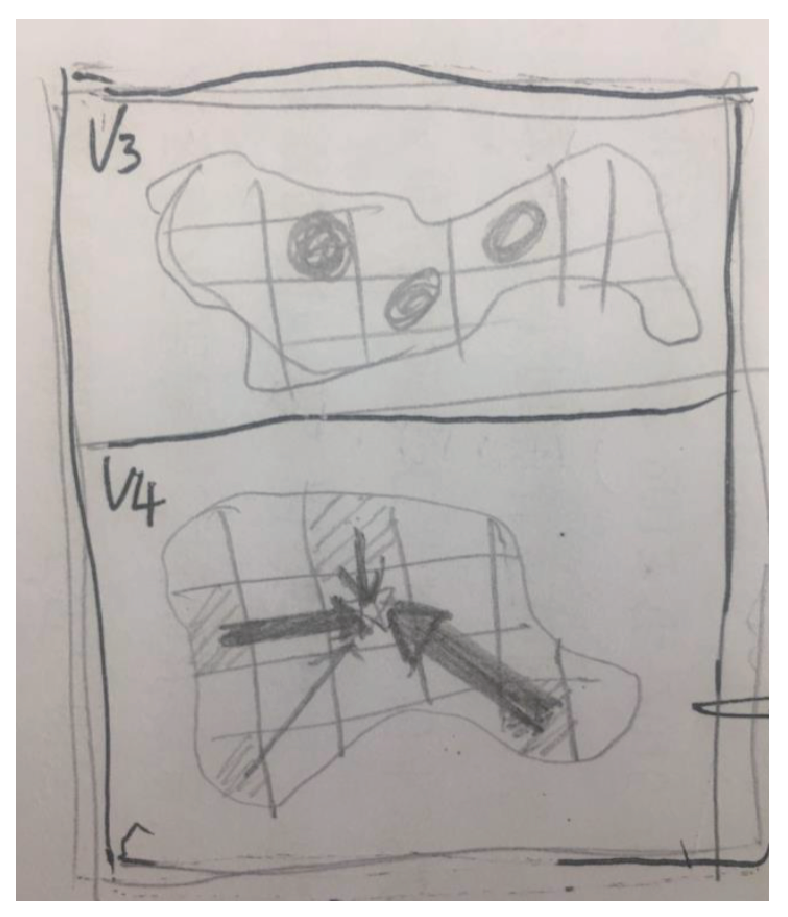
\includegraphics[width=\columnwidth]{pictures/case3draft}
 \caption{Home-work distances of different groups: (a) with different salary levels; (b) with or without house.}
 \label{case3draft}
\end{figure}


\iffalse
\begin{figure}[htb!]
 \centering % avoid the use of \begin{center}...\end{center} and use \centering instead (more compact)
 \includegraphics[width=\columnwidth]{pictures/case2}
 \caption{Home-work distances of different groups: (a) with different salary levels; (b) with or without house.}
 \label{case2}
\end{figure}


Home-work distance is an essential metric in economics, geography, and sociology. It refers to the distance between house and workplace. It is influenced by many factors like transportation, housing, land use, etc. Understanding the home-work distance of a region helps to evaluate whether the region is well planned or not. In this case, we demonstrate our system's help in home-work distance understanding.

Considering income potentially determines where people live, we use income as the characteristics to select three groups, the group over 500K, the group during 200-300K and the group less than 100K. In Figure~\ref{case2}, the height of the bar stands for visiting frequency of the TAZ and its color encodes the average home-work distance, red for close and yellow for far. As Figure~\ref{case2}(a) shows, for all the three groups in different income levels, most of the TAZs have dark red or red color which indicates the home-work distance is generally short, especially in downtown. Only those with less than 100K salary work outside the center, such as the space in the green circle. When comparing the three groups in the downtown area, it is seen that it takes more time to go to work in Futian District as the decrease of the income.

We explore the home-work distance of groups with and without a house.
Figure~\ref{case2}(b) shows the close-up views. It is found that the Nanshan District has a shorter home-work distance for individuals without a house, while Futian District has shorter for those with a house. Nanshan is relatively newer to Futian so that there might be more easily-accessible houses to be rent.
\fi

\section{Conclusion}
\label{sec:conclusion}

This work demonstrates a throughout research flow from data collection, basic analysis to deep visual analysis of mobility patterns with individual characteristics. Considering the irresistible trend in mixing social data and spatial data to solve the urban problem, this work takes one step forward in exploring the relationship between movement and individuals' characteristics, which is rarely touched by previous geo-tagged social media visual analytics. The design of the visual analytic system is driven by three tasks about individuals and mobility patterns. Tapping into our daily experiences, the data-driven profile visualization provides an organic and intuitive representation of individuals. Its effectiveness in identifying similar or abnormal individuals from the mass has been demonstrated. The design of 2.5D spatial visualization continues the exploration of the typical research problem how to visualize spatial information and abstract information together. Although it is not a one-step solution, 2.5D visualization with the detail slicing is able to provide an occlusion-free analysis with spatial context preserved.

Our current research focuses on fundamental facets of the mobility patterns and doesn't draw a strong conclusion on the correlation between mobility pattern and individual characteristics. In next step, more delicate algorithms will be involved to extract high-level mobility patterns, such as the frequent visiting sequence of an individual group, etc. On the other hand, the data we used in this work shows its potential in representing the population. As the next step, research effort can be put into a more serious verification of how small sampled data can represent a large population.

%\begin{acknowledgements}
%If you'd like to thank anyone, place your comments here
%and remove the percent signs.
%\end{acknowledgements}

% BibTeX users please use one of
\bibliographystyle{spbasic}      % basic style, author-year citations
%\bibliographystyle{spmpsci}      % mathematics and physical sciences
%\bibliographystyle{spphys}       % APS-like style for physics
\bibliography{main}
%\bibliography{test}


\end{document}
% end of file template.tex

